\section{Review of Collisions}\index{collisions}

Collisions happen all the time.  Billard balls collide with each other and with the walls of the billiard table.  Cars collide.  People in a crowded room bump into each other.

Collisions are also one of the main ways we study the fundamental forces and particles. In this section, we will review what you learned in high school regarding collisions.  As you may remember, when analyzing what will happen when you collide two objects, conservations laws are very important - especially conservation of energy and conservation of momentum.  You may also remember that there are two classes of collisions: elastic and inelastic.  In an elastic collision, kinetic energy is conserved. In an inelastic collision, the kinetic energy might change due to changes in other forms of energies. Kinetic energy may be changed into heat energy when an object is deformed. Chemical energy might become kinetic energy if something explodes. Both types of collision occur when beams of protons are aimed at each other.

Let's do some simple collisions problems as a review.  If this material is not something you have done before and that you can easily do, then you need to take an introductory physics course before taking this one.

\subsection{Conservation Laws}
Conservation laws are very important in particle physics.  It was proven by Emmy Noether 
(https://en.wikipedia.org/wiki/Emmy\_Noether) 
that for every symmetry of nature, there is a conservation law.  You learned about conservation of energy and momentum during high school. It can be shown that conservation of energy occurs if the laws of physics do not change with time (there is a symmetry relating the laws of physics at different times).  Likewise, conservation of momentum occurs if the laws of physics do not depend on location. Since there are three spatial coordinates, (x, y, and z) there are three separate conservation laws for momentum - one for each component of momentum. 

There are many symmetries between particles. The quarks all look the same to the strong force. All charged particles look the same to the electric force.  Because of this, there are other conservation laws, such as conservation of charge, convervation of baryon number, conservation of lepton number, etc... If you want to learn more about these interesting conservation laws, you'll need to hang in there and take more particle physics as a senior! 

\subsection{Elastic Collisions}

Let's do a simple elastic collision problem as a review. A particle with a speed of 300 m/s collides elastically with another particle at rest. The two particles have the same mass. The first particle leaves the collision at an angle of ${\rm 30^o}$ with respect to its initial direction. What are the speeds of the two particles after the collision and what is the angle of the second particle with respect to the initial direction of the first particle? The problem is summarized graphically in Figure~\ref{fig:elastic}.

 
\begin{figure}[h]
\centering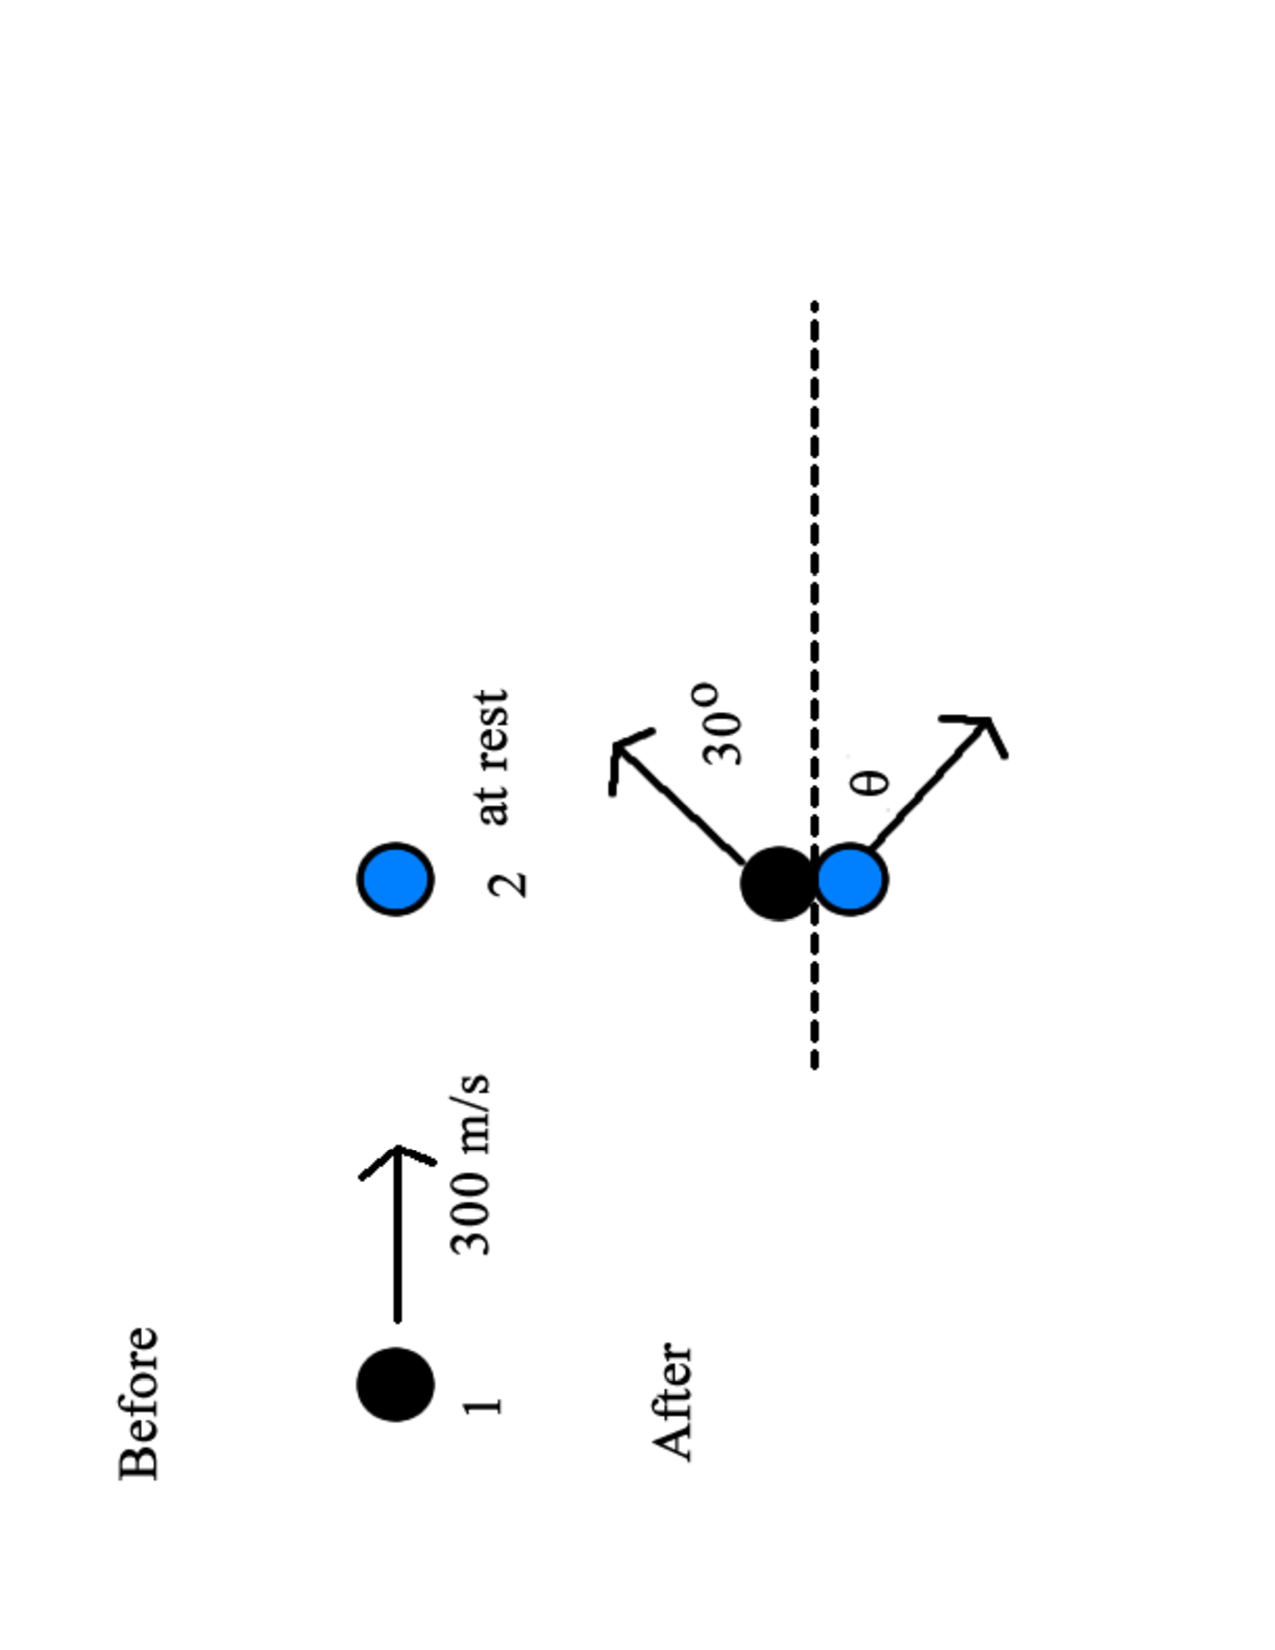
\includegraphics[scale=0.5]{./collisions/Pictures/elastic.pdf}
\caption{cartoon of elastic collision problem}
\label{fig:elastic}
\end{figure}

Let's set our x axis along the initial direction of the first particle, and the y-axis perpendicular to that.  Let's let m be the unknown mass of the two particles, 
${\rm v_{1,f}}$ be the unknown final speed of the first particle,
${\rm v_{2,f}}$ be the unknown final speed of the second particle,
and
${\rm \theta}$ be the unknown final angle of the second particle.
We appear to have four unknowns, but we will see that the $m$ will cancel out of the equations, leaving three unknowns. To solve for three unknowns, we need three equations.  Luckily for elastic collisions, we have three conservation laws.

Using conservation of the x-component of momentum, we have:
$$ m 300 = m v_{1,f} \cos{30} + m v_{2,f} \cos{\theta} $$

Using conservation of the y-component of momentum, we have:
$$ 0 = m v_{1,f} \sin{30} + m v_{2,f} \sin{\theta} $$

Using conservation of kinetic energy, we have:
$$ {1 \over 2} m 300^2 = {1 \over 2} m v_{1,f}^2 + {1 \over 2} m v_{2,f}^2 $$

Can you solve this system of equations?  I hope so.  You should get:
$v_{1,f}=260~m/s$, $v_{2,f}=150~m/s$, and $\theta = 60^o$.

(hint: try solving the first two for 
${\rm v_{2,f} \cos{\theta}}$ and ${\rm v_{2,f} \sin{\theta}}$, 
squaring the resulting equations, and adding them to get rid of the trig functions)

\subsection{Inelastic Collisions}

Let's do a simple inelastic collision problem as review.  Take the same two initial particles.  This time, however, the two particles stick together (some of the energy somehow becomes a kind of binding energy between the two, perhaps also some goes into deformation of the two).  What is the speed and direction of the final combined particle?  The problem is summarized graphically in Figure~\ref{fig:inelastic}.
 
\begin{figure}[h]
\centering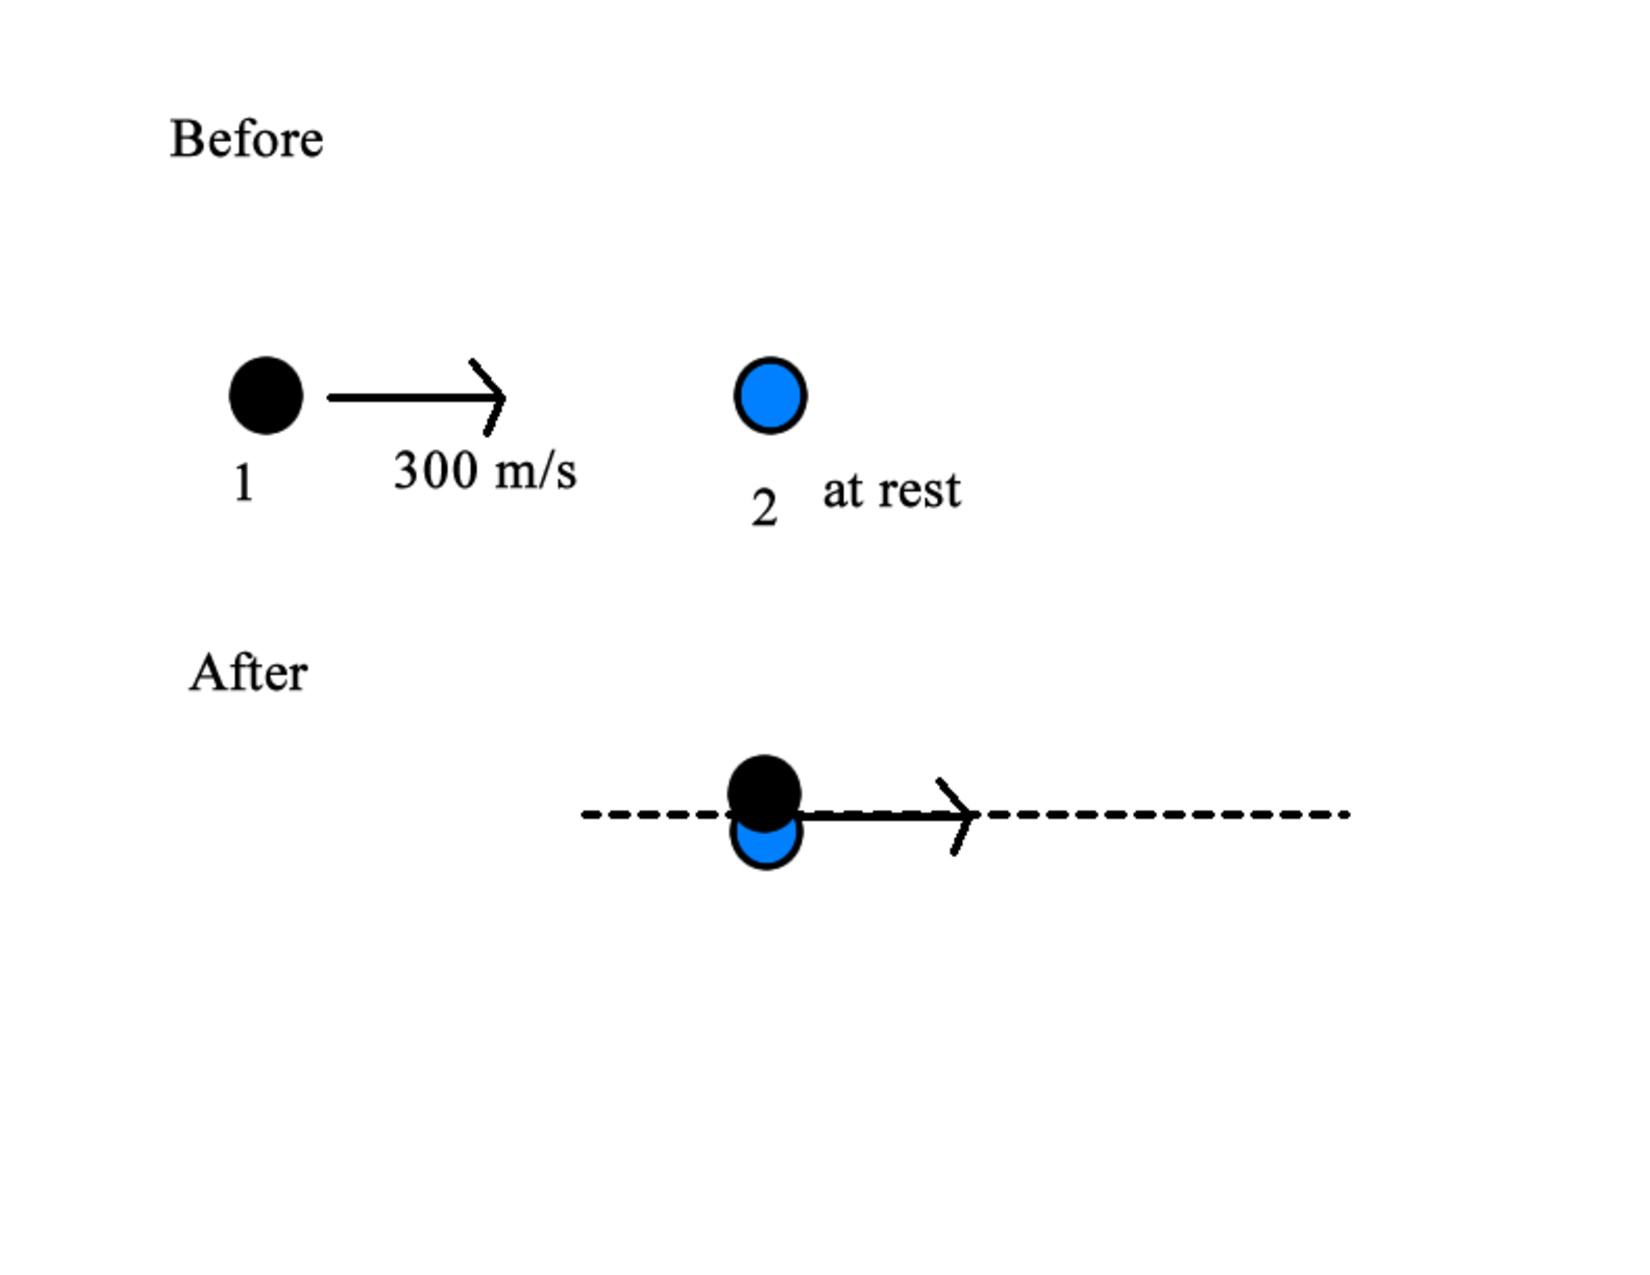
\includegraphics[scale=0.5]{./collisions/Pictures/inelastic.pdf}
\caption{cartoon of inelastic collision problem}
\label{fig:inelastic}
\end{figure}


This should be an easy problem for you. You should get that the velocity of the final combined object is 150 ${\rm m/s}$.
By how much has the total kinetic energy changed?
